\documentclass[12pt]{article}
\usepackage[spanish]{babel}

%%%%%%%%%%%%%%%%%%%%%%%%%%%%%%%%%%
%%%%%%%%%%%%%%%%%%%%%%%%%%%%%   %%
%%        Datos Trabajo     %%  %%
%%%%%%%%%%%%%%%%%%%%%%%%%%%%%%%%%%
\newcommand{\titulo}[0]{Evidencia de aprendizaje: Análisis de datos}
\newcommand{\materia}[0]{Estadística Básica}
\newcommand{\grupo}[0]{BI-BEBA-2002-B2-013}
\newcommand{\unidad}[0]{Unidad 2}


%%%%%%%%%%%%%%%%%%%%%%%%%%%%%%%%%%
%%%%%%%%%%%%%%%%%%%%%%%%%%%%%%%%%%
\usepackage{amssymb}
\usepackage{enumerate}
\usepackage{geometry}
\usepackage{mathtools}
\usepackage{multicol}
\usepackage{soul}

\usepackage{graphicx}
	\graphicspath{ {assets/} }

\usepackage{hyperref}
	\hypersetup{
			pdftex,
		        pdfauthor={bench},
		        pdftitle={\titulo},
		        pdfsubject={\materia},
		        pdfkeywords={\grupo, \unidad, UnADM},
		        pdfproducer={Latex with hyperref, Ubuntu},
		        pdfcreator={pdflatex, or other tool},
			colorlinks=true,
				linkcolor=[rgb]{0,0,0.45},
				urlcolor=cyan,
				filecolor=green,
				citecolor=blue}

%%%%%%%%%%%%%%%%%%%%%%%%%%%%%%%%%%
%%%%%%%%%%%%%%%%%%%%%%%%%%%%%%%%%%

\title{
	
\includegraphics{../../../assets/logo-unadm} \\
	\ \\ Benjam\'in Rivera \\
	\bf{\titulo}\\\ \\}

\author{
	Universidad Abierta y a Distancia de México \\
	TSU en Biotecnolog\'ia \\
	\textit{Materia:} \materia \\
	\textit{Grupo:} \grupo \\
	\textit{Unidad:} \unidad \\
	\\
	\textit{Matricula:} ES202105994 }

\date{\textit{Fecha de entrega:} \today}


%%%%%%%%%%%%%%%%%%%%%%%%%%%%%
%%        Documento         %%
%%%%%%%%%%%%%%%%%%%%%%%%%%%%%%%
\begin{document}
\maketitle\newpage

	\par Antes de continuar, dado el comentario de la \textit{ Evidencia de Aprendizaje } de la primera unidad, en esta actividad exploraremos el campo de profundidad de la base de datos \cite{db}. Esto nos permitirá poder hacer un análisis más adecuado a los temas vistos en la unidad.


\section{Caso de estudio}


	\par Estoy interesado en estudiar las \textbf{t\'ecnicas de repoblaci\'on de ecosistemas} usando agentes biol\'ogicos. Uno de los t\'emas de interes para poder desarrollar esta investigaci\'on es conocer las \textbf{especies por espacio geogr\'afico} que habitan. Esto es importante para poder analizar ecosistemas afectados y aquellos que sean sanos, y que posean caracteristicas similares. 

	\begin{figure}[h]
		\centering
			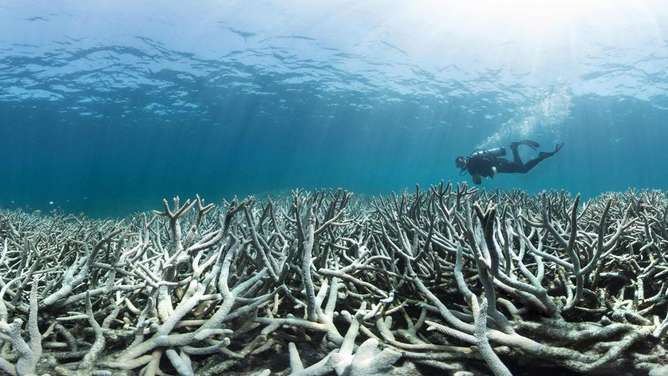
\includegraphics[width=0.6\textwidth]{coral-muerto.jpg}
		\caption{Corales muertos en el Océano Índico por culpa del calentamiento global \cite{corales muertos}}
		\label{fig: corales muertos}
	\end{figure}
	

	\par Entonces en \textbf{esta parte} nos centraremos en las \textbf{ubicaciones de los bancos de algas del mundo}. Esta informaci\'on nos pertmitira teorizar t\'ecnicas de \textit{biorremediaci\'on} en funci\'on de otros ambientes similares. Adem\'as, el estudio de estos en alg\'un tiempo determinado nos dara una oportunidad para identificar causas de infeccion y muerte de las agrupaciones de estos; para tratar de predecir los corales que esten en peligro por causas similares.
	
\section{Base de Datos}

	\par De manera que usando la base de datos \cite{db} obtenemos la visualización preliminar que podemos ver en la figura~\ref{fig: tabla}.
	
	\begin{figure}[h]
	\centering
		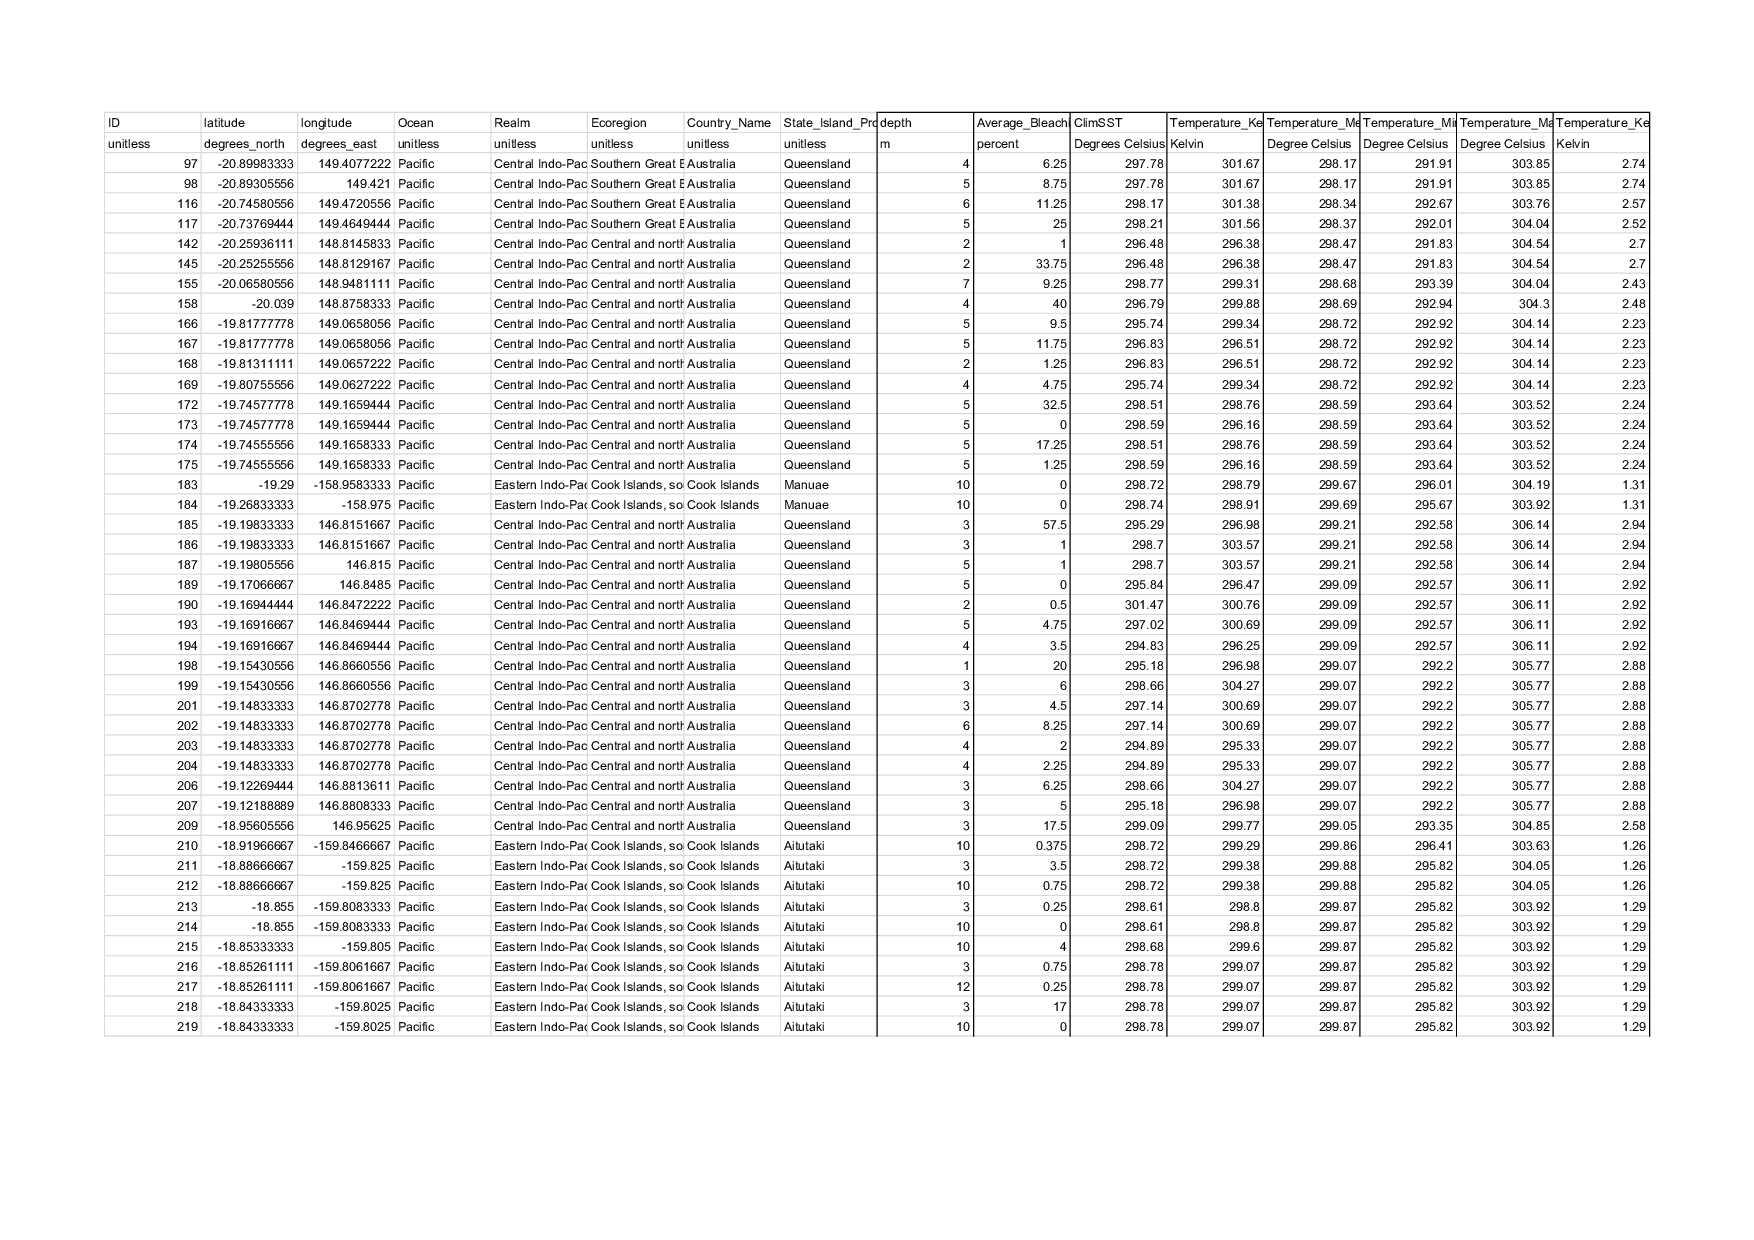
\includegraphics[height=0.6\textheight]{dataset_coral.png}
	\caption{Representación de la información guardada en la base de datos.}
	\label{fig: tabla}
\end{figure}

	
	
\subsection{Tabla}

	\par Con los datos de la columna profundidad\footnote{\textit{depth} porque esta en ingles. } de la figura~\ref{fig: tabla}, obtenemos la tabla de frecuencias de la figura~\ref{fig: tabla frecuencia}. En esta se calcularon la frecuencia absoluta, la frecuencia absoluta acumulada, la frecuencia relativa y la frecuencia relativa acumulada, adem\'as de las clases usadas y los limites, inferiores y superiores, de los datos con los que trabajaremos en este proyecto.
	\par Esta tabla \'unicamente incluirá los primeros 100 datos de la base de datos. Debemos de tener cuidado con esto porque puede ser que estos datos no estén bien distribuidos y podría llevarnos a conclusiones erróneas si son considerados de otra manera.

	
	\begin{figure}[h]
	\centering
		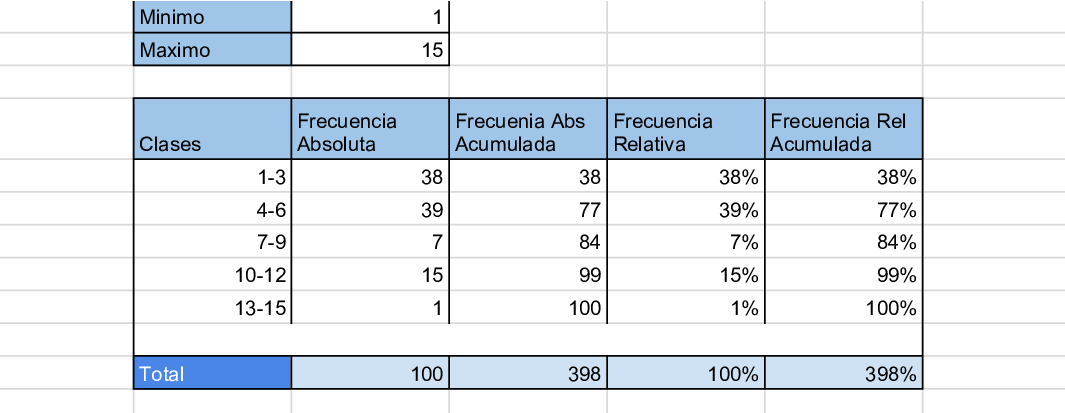
\includegraphics[width=1.0\textwidth]{dataset_coral-frecuencias.png}
	\caption{Tabla de frecuencias de los primeros 100 datos de profundidad de los datos de los corales.}
	\label{fig: tabla frecuencia}
\end{figure}

	

\subsection{Gráficos}

	\par En la figura~\ref{fig: graficos} podemos apreciar los cuatro datos que expresamos en la tabla de frecuencias.
	\par Para las frecuencias absolutas escogí un gráfico de barras porque permite apreciar de manera bruta los datos. Respecto a la frecuencia relativa tome un gráfico circular que permite apreciar de una sola vista la distribución de los datos en el universo. Para ambos acumulados tome una gráfica de puntos y lineas que permite observar como se van acumulando los datos de ambas frecuencias e ir viendo las pendientes entre los datos.
	
	\begin{figure}[h]
	\centering
		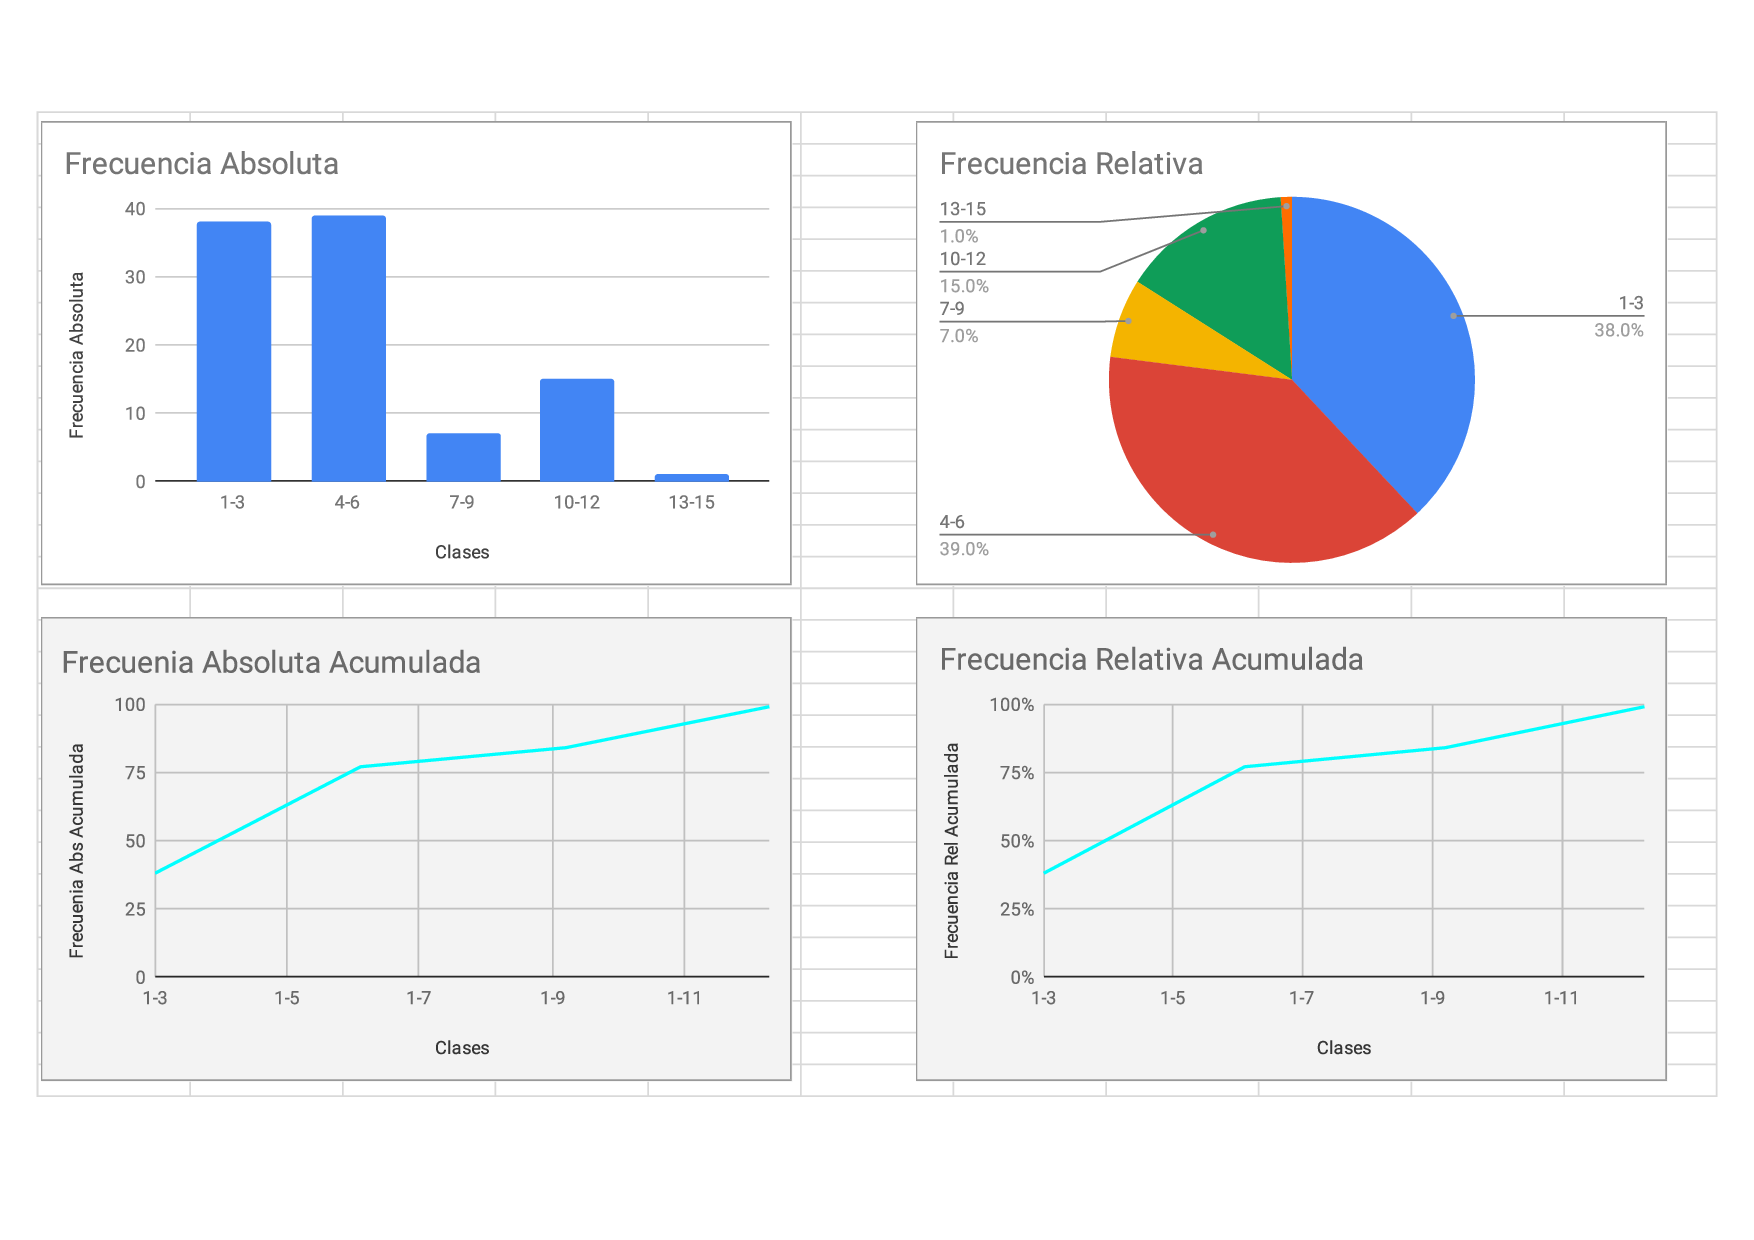
\includegraphics[width=1\textwidth]{dataset_coral-graficos.png}
	\caption{Gr\'aficos generados de la tabla de distribuci\'on de frecuencias.}
	\label{fig: graficos}
\end{figure}





\section{Conclusiones}

	\par Respecto a la representación de datos, es bastante evidente que tanto los gráficos como las tablas ayudan entender mejor los datos con los que se este trabajando.
	\par Respecto a la interpretación de los gráficos, de un análisis externo podemos ver que la mayoría de los datos sobre los que trabajamos corresponden a corales de la zona del mar \textit{ Indo-Pacifico }, principalmente Australia y Figi. 
	\par De estos corales podemos ver que la mayoría están a menos de 6 metros de profundidad, creo que esto puede deberse a la disposición del suelo marino en esta zona, pero requeriría de verificar otros datos para poder corroborarlo. Y de echo, solo tenemos un registro de corales a más de 13 datos de profundidad.
	\par De manera que podemos concluir que en esta zona, las especies nativas de corales, se desarrollan mejor en aguas poco profundas.



%%%%%%%%%%%%%%%%%%%%%%%%%%%%%%%%
%%         Bibliografia        %%
%%%%%%%%%%%%%%%%%%%%%%%%%%%%%%%%%%

\begin{thebibliography}{X}
	\bibitem{EA anterior} Rivera C., B. (2020). \textit{Evidencia de Aprendizaje U1}. No Publicado.
	\bibitem{basico} Universidad Abierta y a Distancia de México. (s/f). \textit{Unidad 2. Representación numérica y gráfica de datos}. UnADM.
	\bibitem{db} van Woesik, R. (2019). \textit{Dataset: Global Bleaching and Environmental Data [Base de Datos]}. Florida Institute of \url{Technology. https://www.bco-dmo.org/dataset/773466}
 
\end{thebibliography}

\end{document}